\documentclass[border=12pt]{standalone}
\usepackage{tikz}
\usetikzlibrary{shapes.geometric, arrows.meta, positioning, calc, fit, backgrounds}
\usepackage{fontspec}
\usepackage{amsmath,amssymb}
\setmainfont{DejaVu Sans}

\begin{document}
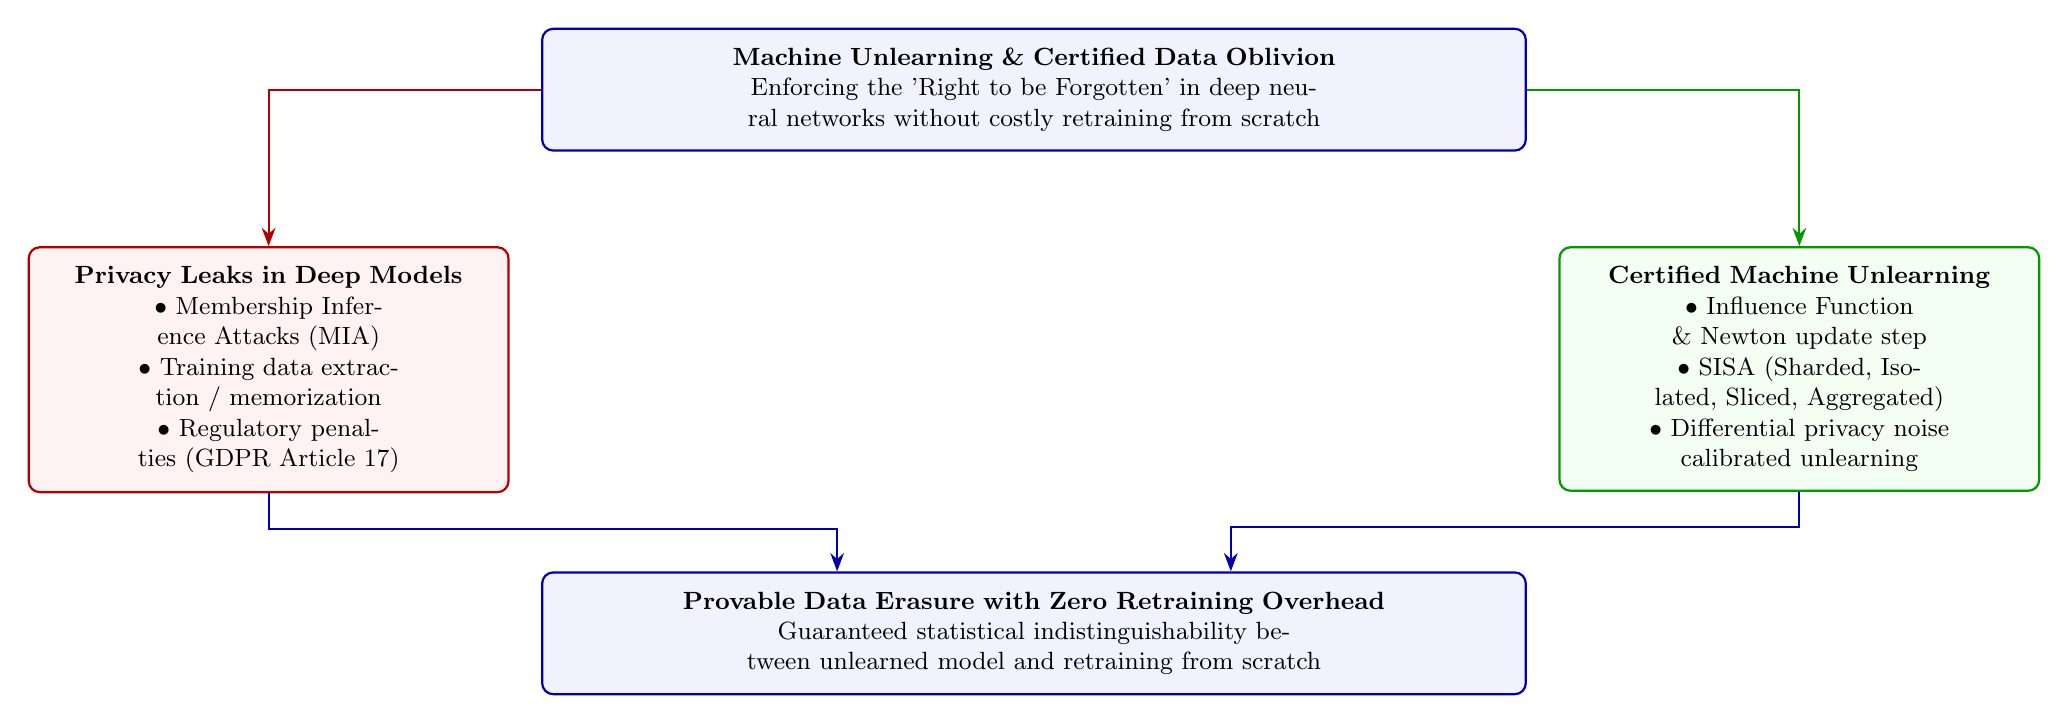
\begin{tikzpicture}[
    font=\small,
    >=Stealth,
    node distance=1.2cm,
    block/.style={rectangle, draw=blue!70!black, fill=blue!5, rounded corners=4pt, thick, align=center, inner sep=7pt},
    alertblock/.style={rectangle, draw=red!70!black, fill=red!5, rounded corners=4pt, thick, align=center, inner sep=7pt},
    greenblock/.style={rectangle, draw=green!60!black, fill=green!5, rounded corners=4pt, thick, align=center, inner sep=7pt},
    amberblock/.style={rectangle, draw=orange!80!black, fill=orange!5, rounded corners=4pt, thick, align=center, inner sep=7pt}
]

\node[block, text width=12cm] (top) {\textbf{Machine Unlearning \& Certified Data Oblivion}\\Enforcing the 'Right to be Forgotten' in deep neural networks without costly retraining from scratch};

\node[alertblock, below left=1.2cm and 0.4cm of top, text width=5.6cm] (privacy_risk) {\textbf{Privacy Leaks in Deep Models}\\$\bullet$ Membership Inference Attacks (MIA)\\$\bullet$ Training data extraction / memorization\\$\bullet$ Regulatory penalties (GDPR Article 17)};

\node[greenblock, below right=1.2cm and 0.4cm of top, text width=5.6cm] (unlearning_tech) {\textbf{Certified Machine Unlearning}\\$\bullet$ Influence Function \& Newton update step\\$\bullet$ SISA (Sharded, Isolated, Sliced, Aggregated)\\$\bullet$ Differential privacy noise calibrated unlearning};

\node[block, below=1.0cm of $(privacy_risk.south)!0.5!(unlearning_tech.south)$, text width=12cm] (bottom) {\textbf{Provable Data Erasure with Zero Retraining Overhead}\\Guaranteed statistical indistinguishability between unlearned model and retraining from scratch};

\draw[->, thick, red!70!black] (top) -| (privacy_risk);
\draw[->, thick, green!60!black] (top) -| (unlearning_tech);
\draw[->, thick, blue!70!black] (privacy_risk.south) -- ++(0,-0.45) -| ([xshift=-2.5cm]bottom.north);
\draw[->, thick, blue!70!black] (unlearning_tech.south) -- ++(0,-0.45) -| ([xshift=2.5cm]bottom.north);

\end{tikzpicture}
\end{document}
